\section {Discussion}

\label{discussion}
\begin{figure*}[tp]
    \centering
    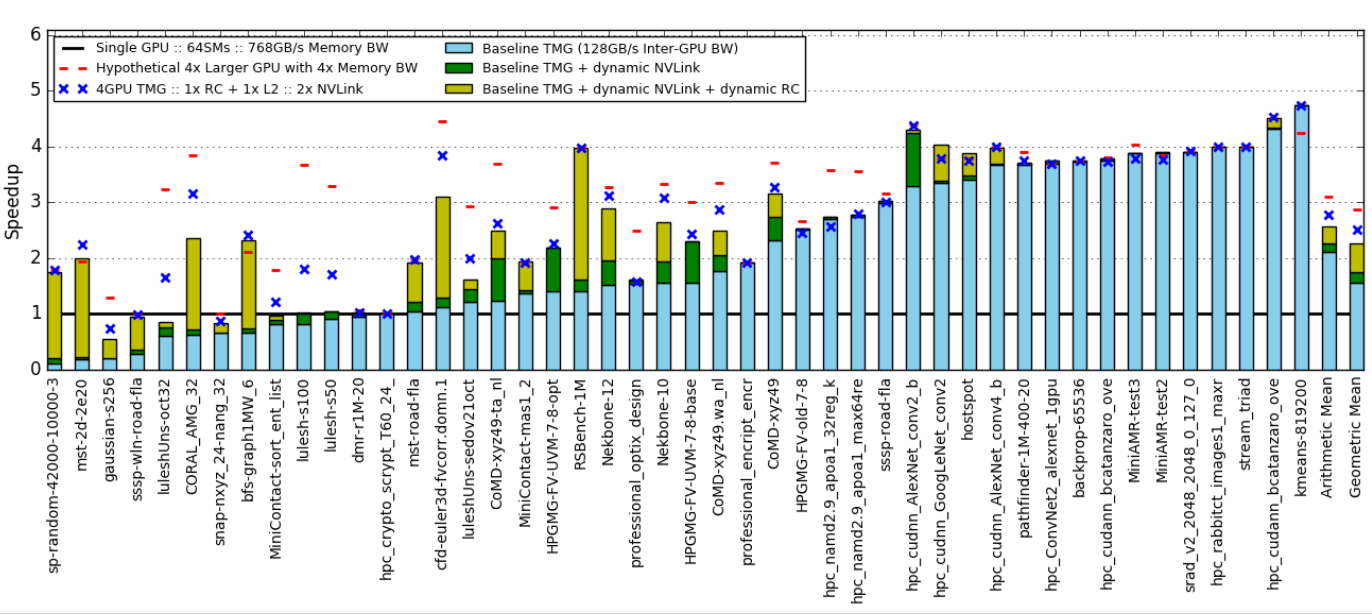
\includegraphics[width=0.9\textwidth]{figures/resultscombined.jpg}
    \caption{Performance of multi-socket GPU with combined assymetric 
optimizations.}
    \label{fig:combined}
\end{figure*}

In Sections~\ref{interconnect} and~\ref{caching} we explored the performance 
implications of dynamically managing GPU interconnect bandwidth and allowing 
individual GPUs to dymnamically allocate on-chip cache capacity to decrease 
dependance on memory system resources when oversubscribed.  Both of these 
techniques aim to more efficiently utilize the available system bandwidth within 
our NUMA multi-GPU system, closing the gap between multi-socket bandwidth and 
local memory bandwidth.  These two techniques are orthoginal and could be 
applied in isolation or in combination.  Dynamic interconnect balancing has an 
implementation advantage in that the system level changes to enable this feature 
are very isolated from the larger GPU, only the link level load balancer on both 
the GPU and switch need to be modified.  Conversely, enabling GPU caching of 
remote memory and dynamic balancing of cache capacity based on interconnect 
utilization requires changes to both the physical cache architectures and the 
GPU coherence protocol.

Because these two features target similar improvements, when employed together 
their effects are not strictly additive.  Figure~\ref{fig:combined} shows the 
improvement when applying both dynamic interconnect and dynamic cache management 
together.  For benchmarks such as \texttt{CoMD}, these features contribute 
nearly equally to the overall improvement, but for others such as 
\texttt{HPGMG} or \texttt{MST}, interconnect improvements or caching are the 
primary contributor respectively.  On average, we observe that when combined we 
see XXX\% improvement in multi-GPU performance when applying our proposed 
optimizations.

\begin{figure*}[t]
    \centering
    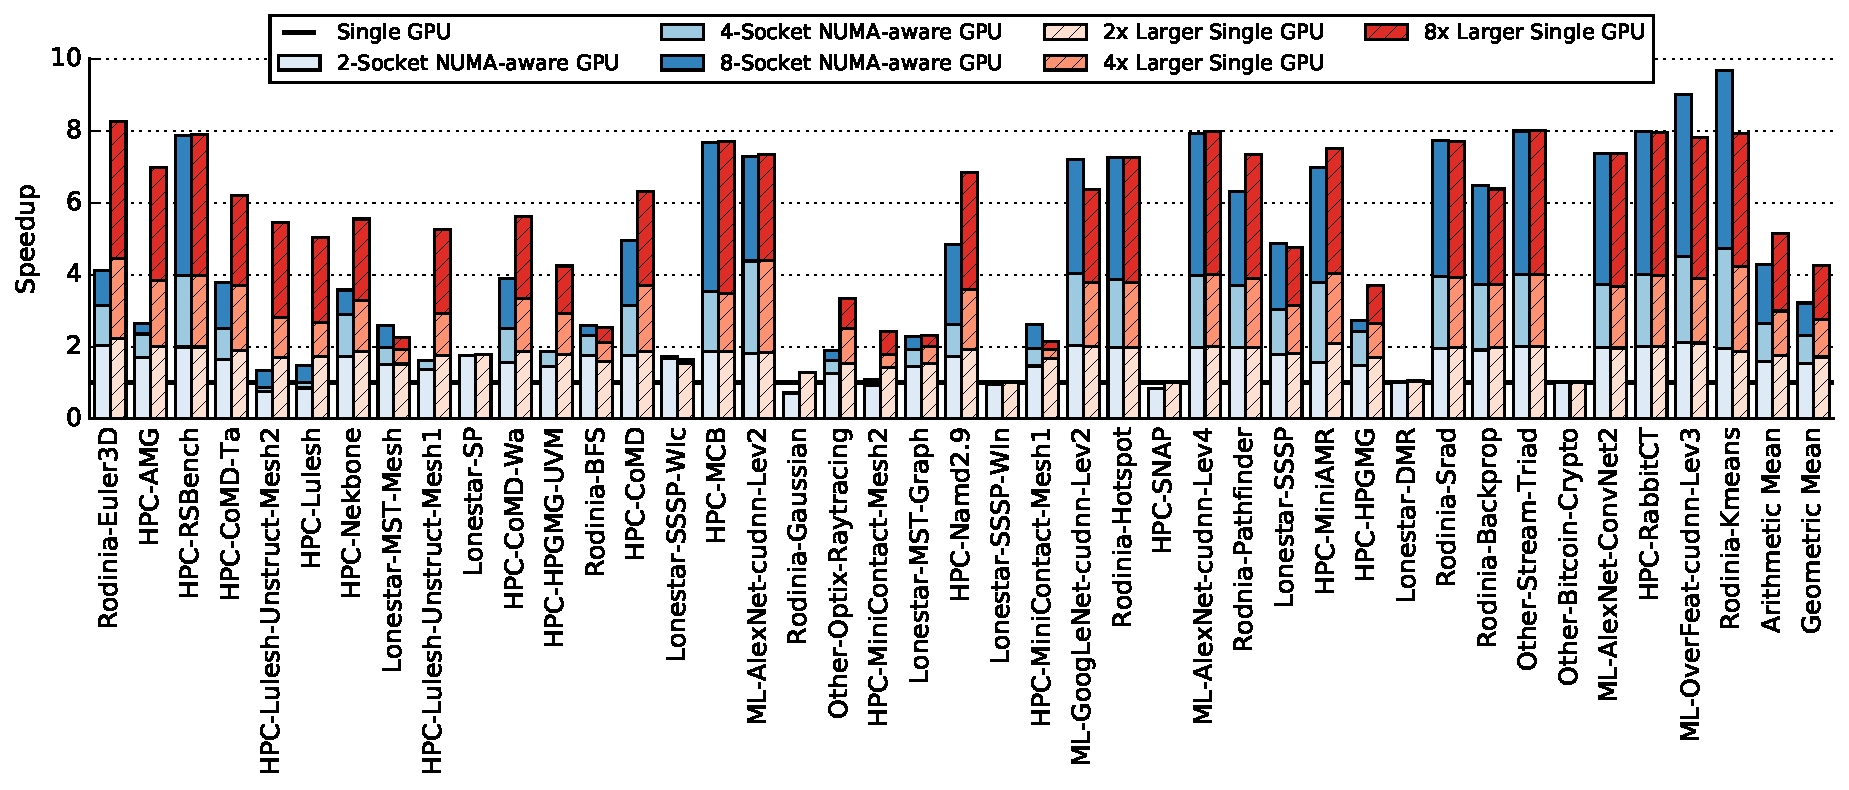
\includegraphics[width=0.9\textwidth]{figures/plot_scalability_mgpu_WB.pdf}
    \caption{Scalability of multi-socket GPU as we move from 1-8 GPUs}
    \label{fig:scalability}
\end{figure*}

\textbf{Scalability:} When considering moving from a single socket GPU to
multi-socket GPU solutions the question arises of what level of efficiency
can be maintained with this approach.  Figure~\ref{fig:scalability} shows the
scalability of a multi-socket GPU approach as we move from a single to 
eight socket multi-GPU implementation.  While larger multi-socket GPUs
may be possible to power and cool within a single node, we observe that due
to parallel efficiency XXX, XXX, XXX.

Another paragraph here once we have results.\vspace{1in}

\textbf{Multi-Tenancy of Large GPUs:} In this work we have shown that many 
workloads today have the ability to
saturate (with sufficient parallel work) a GPU that is at least 4$\times$
larger than today's GPUs.  With deep data becoming commonplace across many
computing paradigms, we believe that the trend of having enough computation
to saturate much larger single GPUs will continue into the forseeable future.
However, when GPUs become larger at the expense of having multiple discrete
GPUs within the system, questions related to GPU provisioning arise.  Applications
that cannot saturate such a GPU will leave resources underutilized and applications
that may be running concurrently in the system currently have to coarse grain
multi-plex the GPU in time cooperatively.  

While not the focus of this work,
there is significant effort in both industry and academia to support finer
grain sharing of GPUs through either shared SM execution~\cite{XXX}, spatial
multi-plexing of a GPU~\cite{XXX}, or through improved time division multiplexing
with GPU pre-emptability~\cite{XXX}.  To support improved per GPU efficiency,
any of these solutions could be applied to a multi-socket GPU to improve utilization
in cases where applications can not fill a significantly larger GPU.  Alternatively,
with additional software work multi-socket GPU designs should be able to be dynamically
partitioned with granularity from 1--N logical GPUs if they are switch connected, providing
yet another level of partitionable flexibility.

\textbf{Power Implications:} \textit{Oreste or Evgeny}
What happens to all the extra bandwidth we need over the interconnect and
power.  we should calculate the extra power but note that even using P2P GPU
access there will still be many remote accesses.  unfortunately we can't quantify
that differential because (drives the point home) there are not multi-GPU versions
for most of our 40+ benchmarks.

% 
% % 
% % One use case in the future
% % may be that GPU programmers will size their application's data to extend well 
% beyond
% % the performance-optimal footprint in CPU and GPU memory.  With excess data 
% spilling over
% % into the additional capacity provided by the CPU memory, performance
% % bottlenecks will shift away from the GPU towards the CPU memory system.  In 
% such
% % cases, the GPU caching policy for CPU memory will come under additional 
% pressure due to
% % the increased traffic skewed towards CPU memory.
% % 
% % To understand how selective caching affects performance under such a scenario, 
% we evaluate
% % a situation wherein the application data has been
% % sized so that 90\% of the footprint resides in CPU memory and just 10\% can 
% fit within GPU memory, as compared to the nearly
% % inverse performance-optimal 20\%-80\% ratio.
% % Figure~\ref{fig:capacityconstrained} shows the performance of this 
% memory-capacity-constrained case relative 
% % to the baseline optimal ratio.  We see that naive selective caching and
% % our proposed enhancements follow the same trend of performance improvements
% % shown previously in Section~\ref{results}.  Because this scenario is primarily 
% limited
% % by the CPU memory system, we see that in some cases the client cache and 
% variable sized transfer interconnect optimizations
% % can actually outperform the hardware cache-coherent GPU due to a reduction in 
% data overfetch between the CPU memory and the GPU client.
% % To validate our observation, we added the same client cache and variable
% % transfers to the hardware cache-coherent baseline configuration and saw an 
% average
% % speedup of 4.5\%.  Whereas the absolute
% % performance achieved, compared to a performance-optimal memory footprint and 
% allocation, may not always be compelling, should
% % software designers chose to partition their problems in this way, we believe 
% selective caching will continue to 
% % perform as well as a hardware cache-coherent GPU.
% % 
% % \begin{figure}[t]
% % 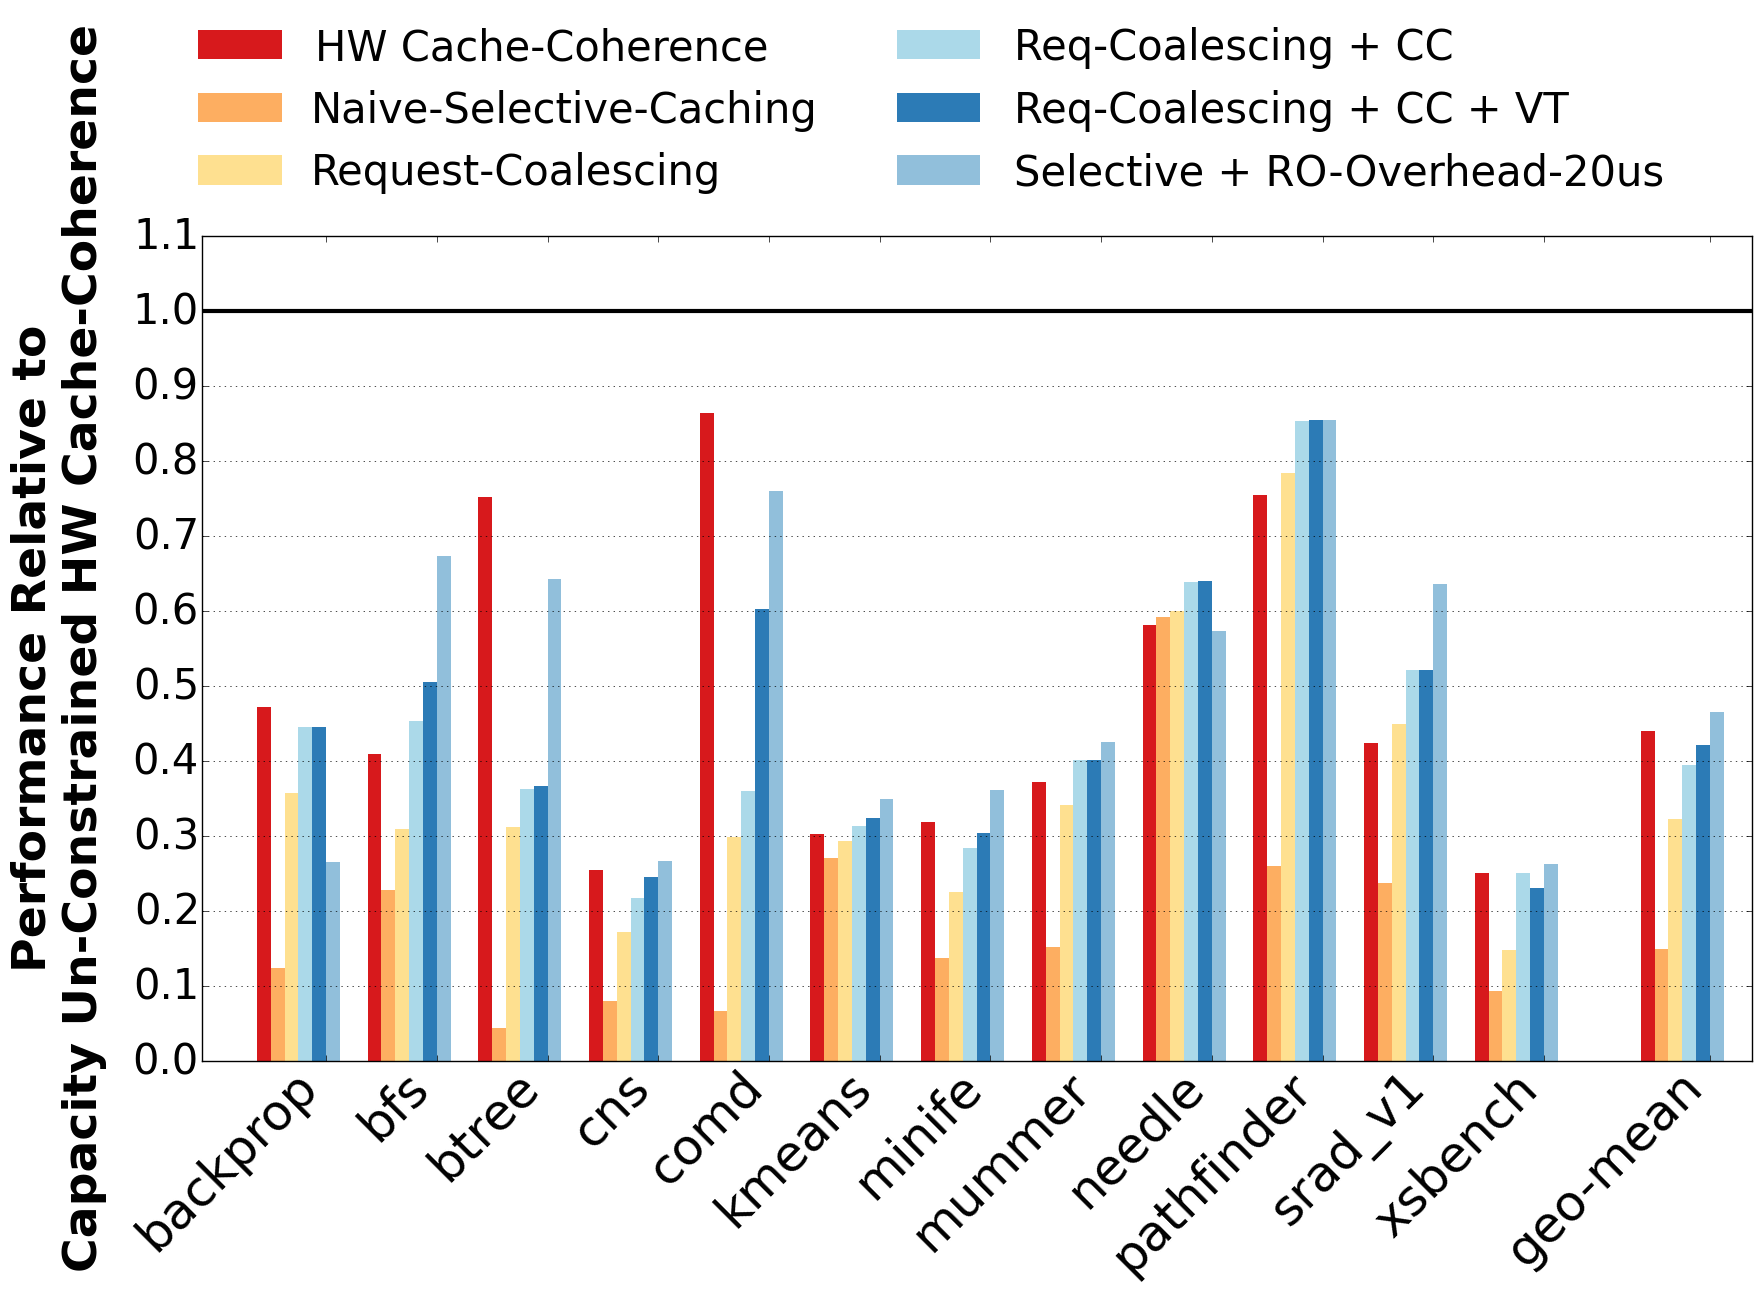
\includegraphics[width=1.0\columnwidth]{figures/capacityconstrained.png}
% % \caption{GPU performance under memory capacity constraints. (CC: Client-Cache,
% % VT: Variable-sized Transfer Units)}
% % \label{fig:capacityconstrained}
% % \end{figure}
% % 
% % In this work, we have primarily investigated a system where bandwidth-aware 
% page placement
% % provides an initial page placement that has been shown to have optimal 
% performance~\cite{Agarwal2015}.
% % Bandwidth-aware page placement is based on the premise that the GPU will place 
% pressure on
% % the CPU and GPU memory system in proportion to the number of pages placed in 
% each memory.  Proposals
% % like selective caching that change the on-chip caching policy of the GPU can 
% cause dramatic
% % shifts in the relative pressure placed on each memory system, effectively 
% changing the bandwidth-optimal 
% % placement ratio.  Although we do not evaluate this phenomenon in this work, 
% balancing
% % initial page placement with dynamic page migration to help compensate for the 
% lack of on-chip
% % caching is an area that needs further investigation.
% % 
% % \section{Related Work}
% % \label{related_work}
% % 
% % Cache coherence for CPUs has received great attention in the literature.
% % Recent proposals have started to explore intra-GPU and CPU--GPU cache 
% coherence.
% % 
% % \textbf{CPU Systems:} Scalable cache coherence has been studied extensively 
% for CPU-based
% %  multicore systems. Kelm et al. show that scaling up coherence to hundreds
% % or thousands of cores will be difficult without moving away from pure
% % hardware-based coherence~\cite{Kelm2009,Hill92}, due to high directory storage
% % overheads and coherence traffic~\cite{Lebeck95,Cheng06}.  
% % Whereas some groups have
% % evaluated software shared memory implementations~\cite{Falsafi94,Hill92}, 
% Martin
% % et al. argue that hardware cache coherence for mainstream processors is here 
% to
% % stay, because shifting away from it simply shifts the burden of correctness 
% into
% % software instead of hardware~\cite{Martin2012}. Nevertheless, disciplined 
% programming
% % models coupled with efficient hardware implementations are still being 
% pursued~\cite{choi2011,Sung2013,Sung2015}.
% % 
% % Self-invalidation protocols have been proposed to reduce invalidation traffic 
% and reduce
% % coherence miss latency~\cite{Lebeck95,Lai2000}. Our selective caching request 
% coalescing scheme uses a similar idea,
% % discarding a block immediately after fulfilling requests pending at the MSHR.
% % Other proposals have classified data into private, shared, and
% % instruction pages and have devised techniques to curtail coherence 
% transactions
% % for private data~\cite{Pugsley2010,Hardavellas2009,Cuesta2011,Ros2012}. We 
% instead classify
% % pages into read-only versus read-write and exploit the fact that read-only 
% data
% % can be safely cached in incoherent caches.
% % 
% % Ros and Kaxiras~\cite{Ros2012} have proposed a
% % directory\hyp{}less\slash{}broadcast\hyp{}less coherence protocol where all 
% shared
% % data is self\hyp{}invalidated at synchronization points. In this scheme,
% % at each synchronization point (e.g., lock acquire/release, memory barrier) all
% % caches need to be searched for shared lines and those lines have to be
% % flushed---an expensive operation to implement across hundreds of GPU caches 
% with data
% % shared across thousands of concurrent threads.
% % 
% % \textbf{Heterogeneous Systems and GPUs:} With the widespread adoption of GPUs 
% as a primary
% % computing platform, the integration of CPU and GPU systems has
% % resulted in multiple works assuming that CPUs and GPUs will eventually become
% % hardware cache-coherent with shared page
% % tables~\cite{power2014,Pichai2014,Agarwal2015,Agarwal2015b}.  CPU--GPU 
% coherence
% % mechanisms have been investigated, revisiting many ideas from distributed 
% shared
% % memory and coherence verification~\cite{Gelado2010,wu2014,Kaxiras2013}. Power 
% et
% % al.~\cite{Power2013} target a hardware cache-coherent CPU--GPU system by
% % exploiting the idea of region
% % coherence~\cite{Cantin2005,Alisafaee2012,Moshovos2005,Zebchuk2007}. They treat 
% the CPU and the
% % GPU as separate regions and mitigate the effects of coherence traffic by
% % replacing a standard directory with a region directory. 
% % In contrast, we identify that CPUs and GPUs need not be cache-coherent; 
% % the benefits of unified shared memory can also be achieved via selective 
% caching, which has lower
% % implementation complexity.
% % 
% % Mixing incoherent and coherent shared address spaces has been explored before 
% in the context of
% % CPU-only systems~\cite{Huh04} and the appropriate memory model for mixed
% % CPU--GPU systems is still up for
% % debate~\cite{Lim2012,Hechtman2014,Hower2014,Gaster2015}.  Hechtman et 
% al.~propose 
% % a consistency model for GPUs based on release consistency, which allows
% % coherence to be enforced only at release operations.  They propose a 
% % write-through no-write-allocate write-combining cache that tracks dirty data
% % at byte granularity.  Writes must be flushed (invalidating other cached 
% copies) only 
% % at release operations.  Under such a consistency model, our selective caching 
% scheme 
% % can be used to avoid the need to implement hardware support for these 
% invalidations between
% % the CPU and GPU.
% % 
% % Cache coherence for GPU-only systems has been studied by
% % Singh et al.~\cite{Singh2013}, where they propose a timestamp-based hardware 
% % cache-coherence protocol to self-invalidate cache lines. Their scheme targets 
% % single-chip systems and would require synchronized timers across multiple 
% % chips when implemented in multi-chip CPU--GPU environments.
% % Kumar et al.~\cite{Kumar2015} examine CPUs and fixed-function accelerator
% % coherence, balancing coherence and DMA transfers to prevent data ping-pong.
% % Suh et al.~\cite{Suh2004} propose integrating different coherence
% % protocols in separate domains (such as MESI in one domain and MEI in 
% another). 
% % However, this approach requires invasive changes to
% % the coherence protocols implemented in both domains and
% % requires significant implementation effort by both CPU and GPU vendors.
% % 
% % \textbf{Bloom Filters:} Bloom Filters~\cite{Bloom1970} and Cuckoo
% % Filters~\cite{Pagh2004,fan2014} have been used by several
% % architects~\cite{Strauss2006,Zebchuk2009,Hongzhou2011} in the past. Fusion
% % coherence~\cite{wu2014} uses a cuckoo directory to optimize for power and area 
% in
% % a CMP system. JETTY filters~\cite{Moshovos2001} have been proposed for 
% reducing
% % the energy spent on snoops in an SMP system. We use a cuckoo filter to 
% implement
% % the GPU remote directory.
